% This is style of APS journal, physicists should aim to use it
\documentclass[prl,12pt,notitlepage,aps,onecolumn,superscriptaddress]{revtex4-1}

%---------------------------------------------------------------
\usepackage{listings} % allow to include nicely formated listings
\usepackage{xcolor}   % we can add and use colors
\usepackage{fullpage} % default article style is to greedy about margins
\usepackage{graphicx} % REQUIRED TO WORK WITH FIGURES
\usepackage{amsmath,amssymb} % much better math and equation handling
\usepackage{booktabs}
\usepackage{float}
%---------------------------------------------------------------

\begin{document}
%---------------------------------------------------------------
\title{Lab 05 Report}
\author{William Laney \& Karen Ficenec}
\date{October 12, 2016}
\maketitle

\section{Group Member Roles}
Resource Manager (collected and tested components): William and Karen

Hardware Specialist (assembled the circuit): William and Karen

Programer: William and Karen

QA Specialist William and Karen

\section{Initial setup and testing}
We began this lab by connecting the MCP3002 analog to digital convertor (ADC) to the raspberry pi using SPI. We used GPIO 08 as the chip select pin. This design came from the Lab 5 instructions. To confirm that the ADC was working correctly, and to discover the bounds of the device we put a DC voltage into input 1 of the MCP3002 and tied input 2 to ground. We then varied the input voltage from 0 to near 3.3V. We did not go over 3.3V because this was the voltage used to power the device, and thus the upper rail. The results of this can be seen in table 1. The plot seen in figure 1 shows the percent error between the voltage input measured by a digital multi meter and the input voltage measured by the ADC. From this we learned that the MCP3002 is less precise when the voltage is near ground, and gains precision until the voltage is about 0.25V, then the it stays constant. This is expected because at low voltages the measured voltage is closer to the noise in the system. We believe that if we placed a capacitor to ground at the Vin pin we could increase the precision of readings at lower voltages.

% Table generated by Excel2LaTeX from sheet 'Sheet1'
\begin{table}[h]
 \centering
 \caption{DC Voltage Readings}
   \begin{tabular}{c|c|c}
   \toprule
   Expected & Observed & Percent Error \\
   \midrule
   0.005 & 0.006 & 0.2 \\
   0.25  & 0.251 & 0.004 \\
   0.513 & 0.512 & 0.001949318 \\
   0.723 & 0.728 & 0.006915629 \\
   1.042 & 1.044 & 0.001919386 \\
   1.265 & 1.267 & 0.001581028 \\
   1.542 & 1.54  & 0.001297017 \\
   1.738 & 1.74  & 0.001150748 \\
   2.102 & 2.104 & 0.000951475 \\
   2.275 & 2.275 & 0 \\
   2.539 & 2.539 & 0 \\
   2.799 & 2.8   & 0.00035727 \\
   3.061 & 3.062 & 0.000326691 \\
   3.188 & 3.184 & 0.001254705 \\
   \bottomrule
   \end{tabular}%
 \label{tab:addlabel}%
\end{table}%

\begin{figure}[h]
\begin{center}
\includegraphics[width=.5\columnwidth]{plot.png}
\end{center}
\caption{\label{fig:pic} Percent error graph}
\end{figure}

\section{Creating a Scope}
Next we wrote code that would recored a series of data points and plot them. This allows use to see how voltage varies at time and look at waveforms. We found through experimentation that recording about 1000 data points at the maximum sampling frequency of the Pi led to the best results. In addition to recording and plotting data we created code that would use an external trigger to begin the data sampling. We used an interrupt service routine that waited for a rising edge to trigger. We then connected the TTL to the interrupt pin and used this to trigger our scope. On a sine wave the TTL sends a high pulse at the beginning of the rising part of the sin wave. Due to speed constraints of the pi this caused it to begin sampling data normally somewhere near the peak of the sin wave. The code we used, with the modification discussed below for speed improvements, in the scope can be seen in listing 1, in the appendix. A picture of our set up can be seen in figure 2.

\begin{figure}[h]
\begin{center}
\includegraphics[width=.5\columnwidth]{cir_pic.jpg}
\end{center}
\caption{\label{fig:pic} Scope circuit}
\end{figure}

Now that we had a working scope with an external trigger we started to try to determine the maximum frequency it could accurately recorded. We found that the maximum frequency was about 350 Hz. Figures 3, 4, and 5 show 40hz 350hz, and 1.08khz respectively. These figures show that as the frequency of the input goes up the pi can no longer sample enough points to make a smooth curve. While at the higher frequencies it may still be possible to accurately calculate the frequency of the wave we do not believe that this corresponds to an operating scope because no information can be provided about the waveform of the input.

\begin{figure}[h]
\begin{center}
\includegraphics[width=.5\columnwidth]{40sin.png}
\end{center}
\caption{\label{fig:pic} 40hz}
\end{figure}

\begin{figure}[h]
\begin{center}
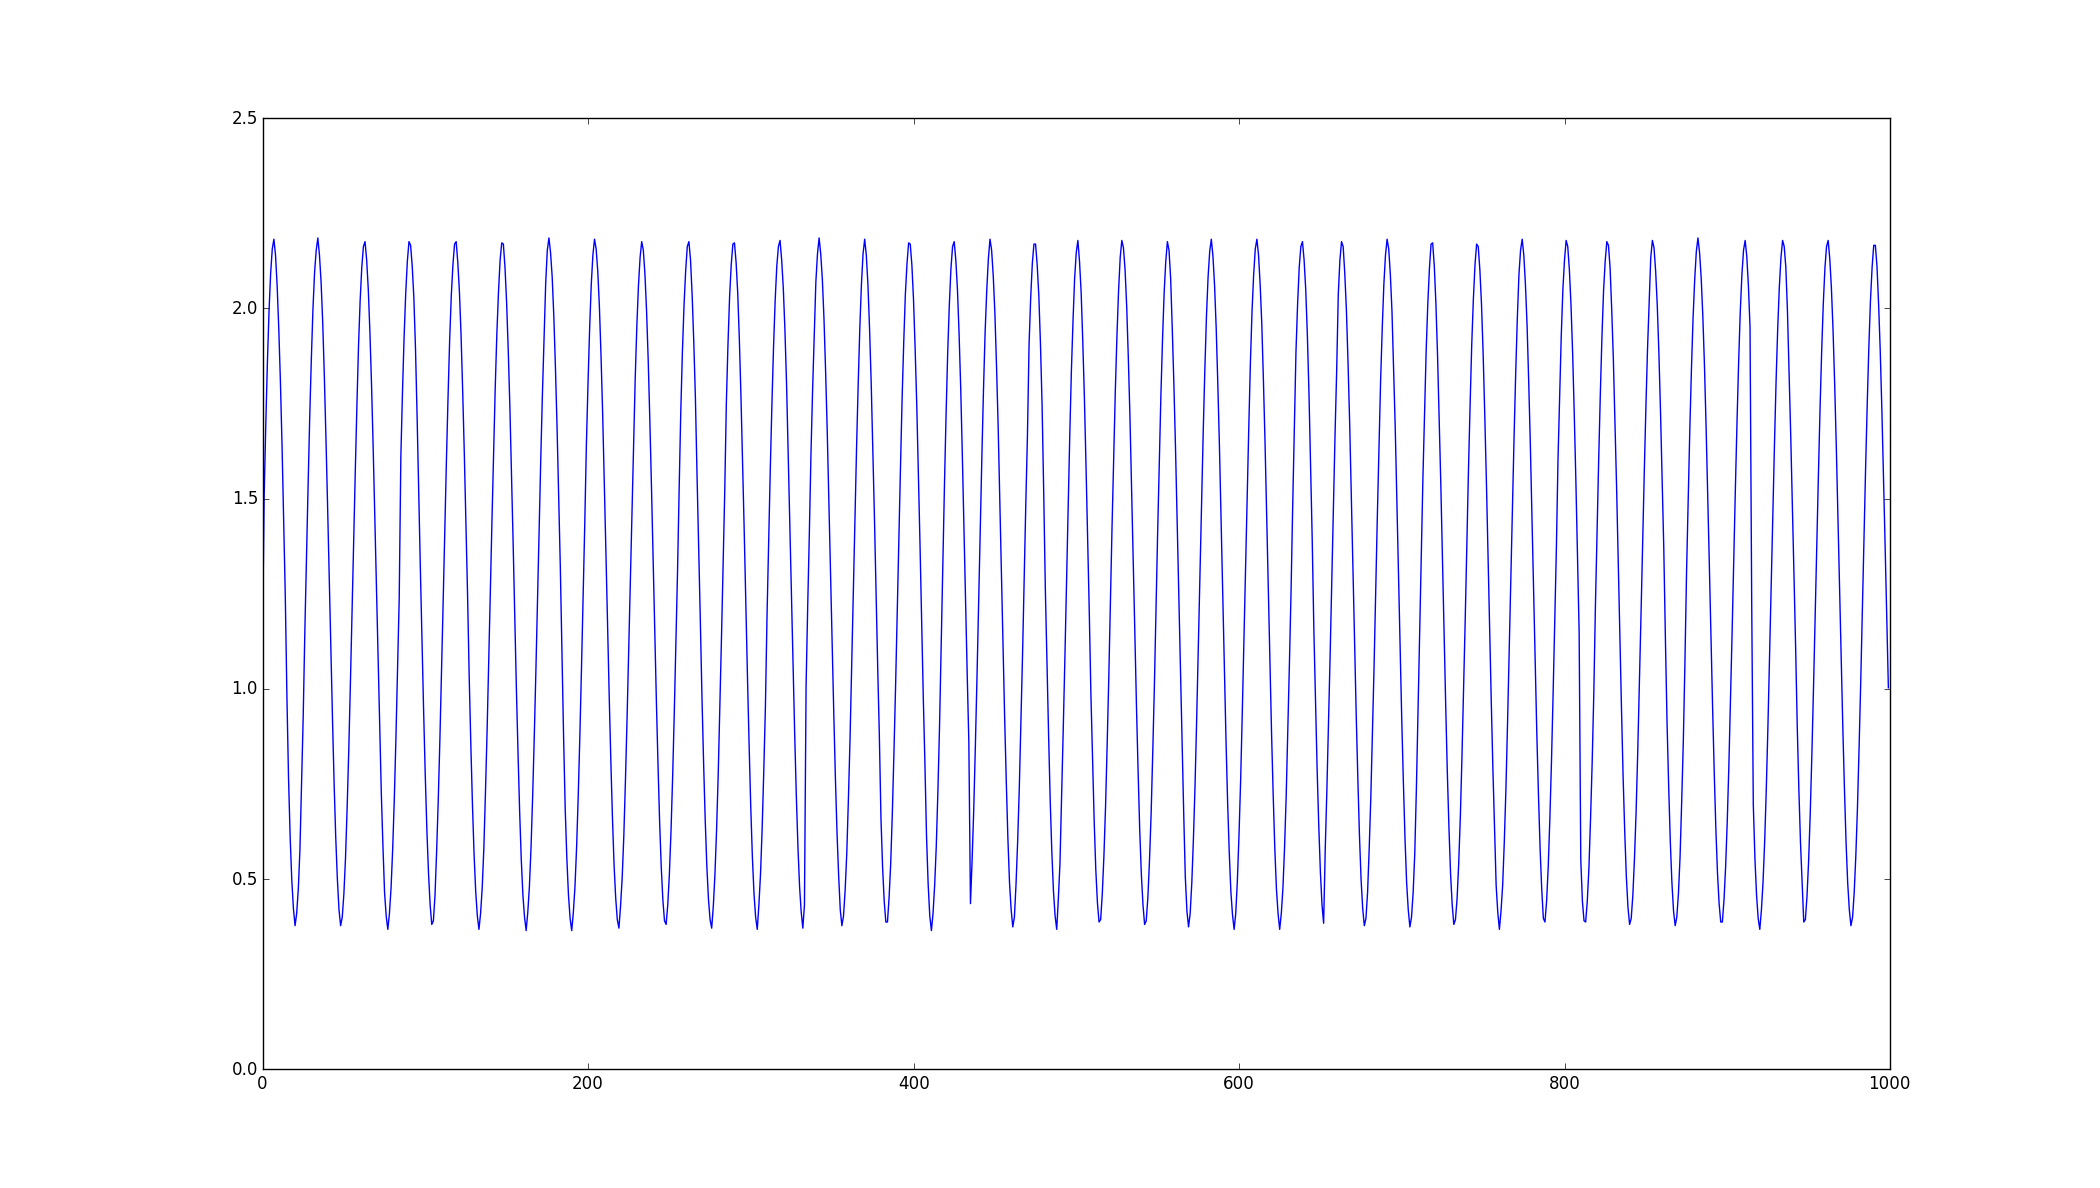
\includegraphics[width=.5\columnwidth]{350_max_freq.png}
\end{center}
\caption{\label{fig:pic} 350Hz}
\end{figure}

\begin{figure}[h]
\begin{center}
\includegraphics[width=.5\columnwidth]{1k08.png}
\end{center}
\caption{\label{fig:pic} 1.08kHz}
\end{figure}

With this maximum found we tried to improve the scope. To do this we began to preallocate memory for storing the data points. In our original code each data point was added on to the end of a list in each iteration of the loop. This meant that each loop iteration the size of the list changed and the system had to change memory allocation to accommodate this. By creating a list of summary values before the loop and then replacing the dummy values with real data the system does not need to change memory allocation with every interaction. This lead to us seeing a better looking waveform at 350Hz, as can be seen in figure 6.

\begin{figure}[h]
\begin{center}
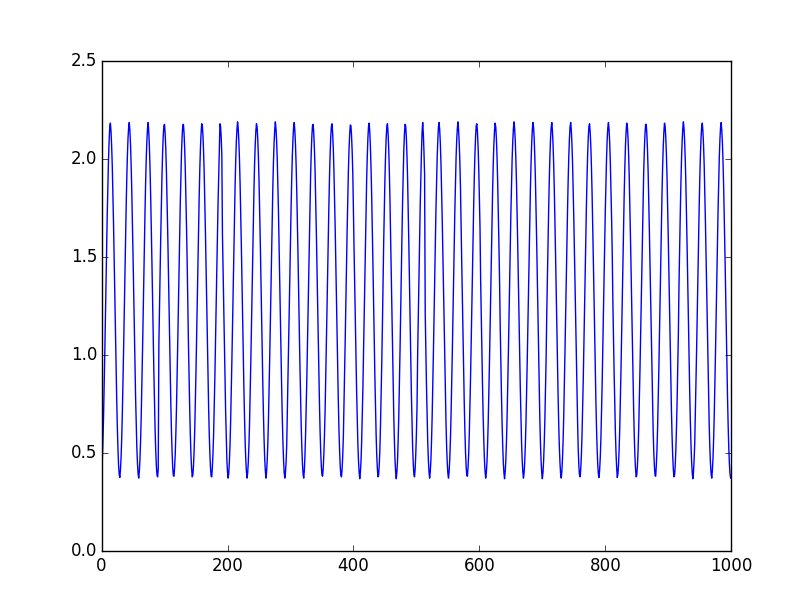
\includegraphics[width=.5\columnwidth]{350_array_good.png}
\end{center}
\caption{\label{fig:pic} 350Hz with memory pre-allocation improvements}
\end{figure}

\section{Conclusion}
In this lab we began by learning about the SPI communication standard. We then learned about how ADCs function. After that we learned how to use python to create plots. Finally we learned how to use external triggers with the Pi to begin executing code.

\section{Appendix}

\lstinputlisting[language=Python, caption=Scope Code, label=amb]{cook_bb.py}

\end{document}